\documentclass{subfiles}

\begin{document}



The aim of this section is to give a practical and scientific insight into the acquisition of data, because a good knowledge of these methods and their limitations is essential for understanding the related research undertaken. The relations between the two main datasets used in this project are depicted on Figure \ref{fig:dataInstrumentsRelations} and briefly explained here: 
\begin{itemize}
\item The \textbf{New Forest dataset} from the UK was provided by the Natural Environment Research Council’s Airborne Research Facility (NERC ARF).  Measurements were collected simultaneously a Leica ALS50-II LIDAR and AISA Eagle/Hawk hyperspectral radiometers on the 8th of April in 2010.  It contains Discrete LiDAR, FW LiDAR and hyperspectral images. 
\item The \textbf{RedGum dataset} was acquired in Australia using a Trimble AX60 integrated LIDAR/Camera instrument over the time period from the 6th of March in 2015 until the 31st of March in 2015.  It was provided by the RPS Australia East Pty Ltd.  Only the FW LiDAR data are used here. 
\end{itemize}

The ALS data are explained first, because they are the main focus of this research, and hyperspectral imagery is towards the end of the chapter. In Section \ref{sec:ALS}, an in-depth description of ALS systems and the differences between discrete and FW LiDAR data is given.  Section \ref{sec:LAS1_3_specifications} briefly discusses the binary file format of the acquired LiDAR data and Section \ref{sec:LeicaVsTrimble} is a discussion on the limitations, the differences and the advantages of two LiDAR instruments; the Leica and Trimble. The essential information about the hyperspectral imagery, which is only associated with the New Forest dataset, is then covered in Section \ref{sec:HyperspectralImages}. 


\begin{figure}[!htbp]
	\centering
	\includegraphics[width=\textwidth]{img/Data_n_Instruments}
	\caption{Data and Instruments}
   	\label{fig:dataInstrumentsRelations}
\end{figure}


\begin{figure} [!htbp]
\centering
\begin{subfigure}[t]{.5\textwidth}
  \centering
  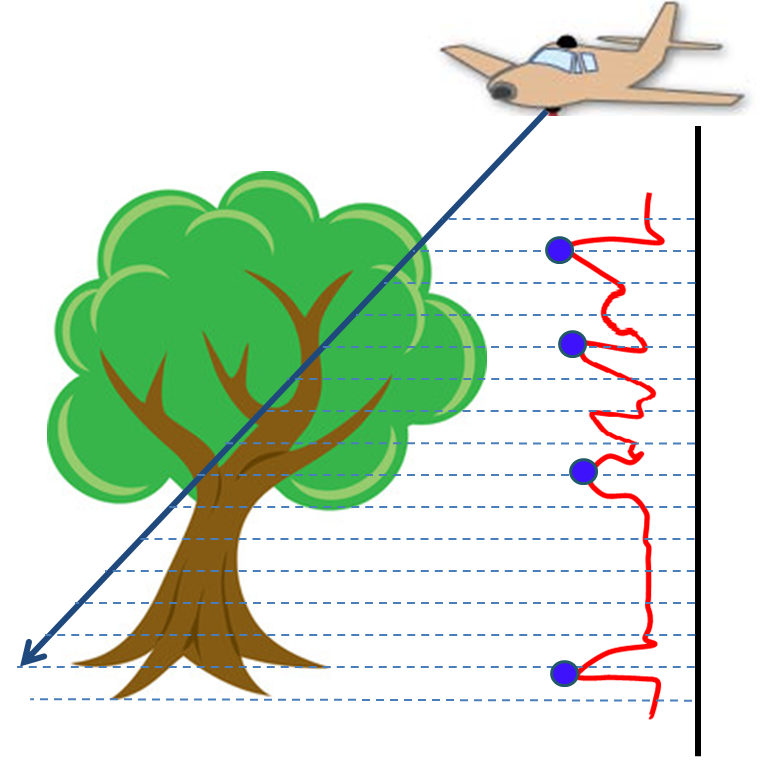
\includegraphics[width=.9\linewidth]{img/LiDAR_DiscretVsFW_fig}
  \caption{A Pulse: Discrete Vs Full-Waveform}
  \label{fig:ALS_pulse}
\end{subfigure}\hfill
\begin{subfigure}[t]{.5\textwidth}
  \centering
  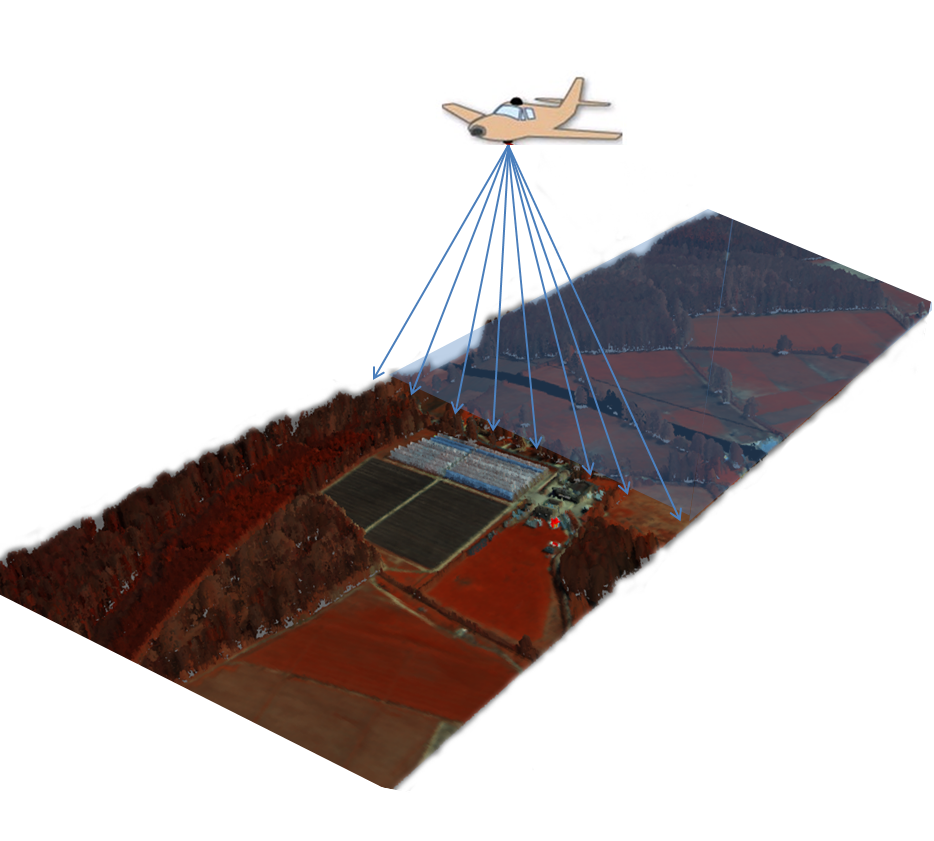
\includegraphics[width=\linewidth]{img/Flightline2}
  \caption{A Flightline}
  \label{fig:ALS_flightline}
\end{subfigure}\hfill
\caption{Airborne Laser Scanning System}
\label{fig:ALS_system}
\end{figure}
%	\footnotemark}
%	           	\footnotetext{Tree image was retrieved from http://images.clipartpanda.com/tree-clip-art-Kij4jKriq.jpeg on 7th o f June. The plane image was retrieved form http://gmv.cast.uark.edu/wp-content/uploads/2013/01/ALS\_scematic.jpg on the 6th of June} 




    \section{Airborne LiDAR systems: An in-depth Explanation}\label{sec:ALS}
     
        
    
    The ALS systems emit laser pulses from sensor mounted in a plane and collects information from the time-of-flight and the returned laser intensity.  By the time the pulse has travelled the approximately 1-3km from the aircraft to the ground, it is roughly 20cm in width due to beam divergence.  When the pulse hits an object (e.g. the forest canopy), then some of it reflects back while the rest penetrates through holes between leaves and branches. The laser pulse continues to hit structures, scattering and partially returning to the sensor until it reaches a solid barrier such as the ground and is fully blocked from further progress.  The LiDAR systems record information from the backscattered laser pulse, measuring its round trip time and the returned intensity.
     
     As mentioned at Section \ref{Background}, there are two types of LiDAR data,  discrete and FW. The discrete LiDAR observes the returned intensity signals and records a few peak intensity returns of the signal, while the FW LiDAR system digitises and stores the enitre backscattered signal into equally spaced time intervals (Figure \ref{fig:ALS_pulse}). The delivered data for the discrete LiDAR is a set of hit points ("returns"), which are associated with laser intensities. The world position of every return is calculated by measuring the round trip time of the laser return, giving a distance from the sensor, which is combined with the precisely known position and orientation of the aircraft/sensor (from GPS, an inertial measurement unit and precise shot direction of the laser pulse). The waveform recordings are triggered by and attached to first returns of discrete LiDAR data (to avoid sampling the uninteresting time period while the pulse travels through the atmosphere) and they are a list of intensities that correspond to the laser intensity returned over time. There is also an offset vector which defines the distance and direction between each wave sample (effectively a compression mechanism, which avoids recording the world position of every sample by replacing it with the location of the first return and this vector).
     
	As shown in Figure \ref{fig:ALS_flightline}, the pulses are scanned back and forth across the landscape below (by a rotating mirror) as the plane travels forward.  The scanned data has a limited maximum width according to the flight height and the field of view scan angle. During processing the track of the plane is divided into easier-to-handle pieces (flightlines) and saved into separate binary files. In this project the LAS1.3 file format is used for both datasets. 
      
     
    \section{Brief Description of the LAS1.3 File Format} \label{sec:LAS1_3_specifications}
    
    \par There are a few LiDAR file formats but the LAS1.3 was the first format to contain FW data and it is the one used to store the data for both  New Forest and RedGum datasets. According to the LAS1.3 file specifications \cite{LAS1.3specifications}, a .LAS file contains information about both discrete and FW LiDAR data, with the waveform packets attached to discrete returns and saved either internally at the end of the .LAS file or externally in a .WVS file. 
    
    \par As shown at (Figure \ref{fig:LAS1_3_fileFormat}) the .LAS file is divided into four sections and a brief explanation of each section is given here:
    \begin{enumerate}
    \item  The \textbf{Header} contains general information about the entire flightline. For example, it includes the maximum scan angle used during the flight, whether the waveform packets are recorded internally or externally  and the number of \textbf{Variable Length Records (VLR)}. 
    \item Regarding the \textbf{VLR}, which contain arbitrary "extension" data blocks, the most important information given is the waveform packet descriptors that contain essential information on how to read the waveform packets (i.e. an ID, the number of wave samples and the size of each intensity in bits). 
    \item The \textbf{Point Data Records} are the discrete points and the waveforms are associated with first return discrete points. Each Point Data Record has a spatial location, an intensity and optionally a pointer to a waveform packet as well as the ID of the corresponding waveform packet descriptor. 
    \item The waveform packets is a list of intensities and they are either saved internally into the \textbf{Extended Variable Length Records} section of the .LAS file or inside an external .WVS file. Starting from the associated first return point, the spatial locations of the waveform packet (wave sample intensity) are calculated by adding an offset defined in the associated Point Data Record. 
    \end{enumerate}  
    

	 \begin{figure}[!htbp]
           \centering
           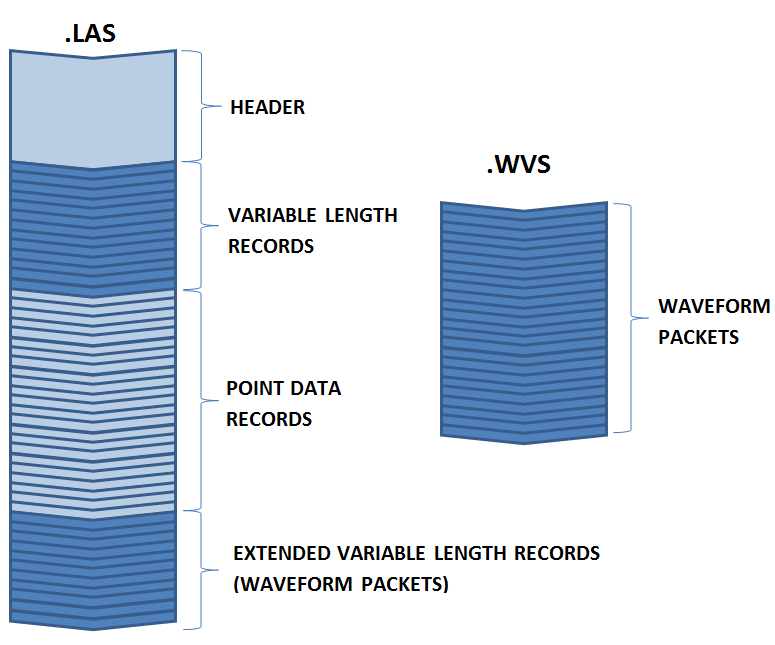
\includegraphics[width=\textwidth/3*2]{img/LAS1_3_fileFormat}
           \caption[LAS1.3 File Format]{How the FW LiDAR data are stored into a binary file, according to the LAS1.3 file format specification }
           \label{fig:LAS1_3_fileFormat}
      \end{figure}

	\section{Leica Vs Trimble Instruments: Limitations, Differences and Advantages}\label{sec:LeicaVsTrimble}
	
	
	\par As shown in Figure \ref{fig:dataInstrumentsRelations}, the Leica ALS 50-II instrument was used to capture the LiDAR data of New Forest dataset and the Trimble AX60 for collecting the RedGum Forest FW LiDAR data. It is therefore important to clarify the differences, the limitations and the advantages of each instrument. 
	
	\par The Trimble performs at a pulse frequency of 400kHz, while the Leica's maximum pulse frequency is 120kHz. Nevertheless, during experiments there were occasions when the Leica discarded every other waveform due to I/O limitations despite being at or below the maximum pulse frequency \cite{Warren2012}. The New Forest dataset has been affected by this and, on average, one third of the saved pulses only contain discrete data. We should therefore be extremely careful when comparing Discrete with FW LiDAR data. While \cite{Anderson2015} concludes that FW LiDAR data worth the extra processing because they have a better vertical profile, \cite{Sumnall2016} states that extra information (the echo-width) from the FW LiDAR data are relatively unimportant. But the New Forest datasets were used for the comparison at \cite{Sumnall2016} and there is no mention about the significantly less waveforms recorded in comparison to the discrete data. It is therefore suspected that their results has been affected by the missing waveforms. 
	
	\par Another problem with the Leica sysyem is the small dynamic range of intensities due to the number of bits used for recording them; the Leica system uses 8-bit integers (0-255 range) while the Trimble uses 16-bit integers (0-16385 range). For increased dynamic range and finer intensities without doubling storage costs, Leica introduced an Automatic Gain Controller (AGC). The AGC is an 8-bit number that defines how the recorded intensity range is shifted across a wider range of intensities. The AGC value is adjusted according to the reflected laser intensity of the previous 64 pulses and it therefore varies across a flightline. Consequently, the raw intensities are incomparable to each other and, since the relation between AGC and the intensities is not linear, the range normalisation is complicated \cite{Lehner2011}\cite{Korpela2010}. In this thesis, the intensities of the Leica system are used as boolean values (whether something existed or not, using a user-defined threshold) to quickly overcome that issue and focus on the major research objectives. Regarding the Trimble instrument, there is no AGC value because the intensities are saved into a 16bit integer and as long as the flight height is constant no normalisation is required. In a few words, the raw intensities recorded using the Leica system are not normalised and therefore not comparable to each other, while the intensities of the Trimble instrument are more meaningful. 
	
	\par The footprint of the laser on the ground depends on the scanning pattern of the instruments and the field of view. The sinusoidal scanning pattern of the Leica system results in a higher density of returns at the edges of the flightline. The footprint of the Trimble instrument is more equally spaced because they are scanned using a rotating polygon. The uneven density pattern of the Leica system is resolved by normalisation during the voxelisation process, but the Trimble's equally spaced pulse pattern is more prone to aliasing when voxelised. Regarding the field of view, the Leica is wider but both systems avoid large angles because otherwise data look deformed at edges of the flightlines. 
	
	\par Last but not least, the Trimble instrument is a native full-waveform sensor; the discrete LiDAR are produced by extracting peak points in post-processing. Therefore one of the purported advantages of a FW system, the concept of extracting a denser point clouds using Gaussian decomposition \cite{Wanger2004}, does not apply in the Trimble's case.  This was proven by extracting peak points from Trimble FW LiDAR data using the pulseextract from LAStools ~\cite{LAStools}; the number of points extracted was exactly the same as the number of points saved into the associated discrete LiDAR files. Therefore discrete data from the Trimble instrument are the same as those generated by echo decomposition and peak points extraction from the FW samples. 
	
	To sum up, the Trimble AX60 instrument is a newer sensor and therefore has less problems or design compromises in comparison to the Leica ALS50-II instrument. Table \ref{tab:InstrumentsSpecs} summarises the differences between the two sensors. 
	
	\begin{table}[!htbp]
		\caption{Specifications of the LiDAR instruments used}
		\label{tab:InstrumentsSpecs}%
		\centering
		\begin{tabular}{|l||m{\textwidth/4}|m{\textwidth/4}|}
			\hline
			\textbf{Instrument Name:}	& \textbf{Leica ALS550-II}     & \textbf{Trimble Ax60  }    \\
			\hline\hline
			\textbf{Scanned Area} & New Forest, UK & RedGum, Australia \\
			\hline
			\textbf{Year of Introduction: }&Discrete LiDAR 2009 \& FW LiDAR 2010& 2013  \\
			\hline
			\textbf{Max Scan Frequency (kHz):} & 120 & 400  \\
			\hline
			\textbf{Recorded Intensity (bits):} & 8 & 16 \\
			\hline
			\textbf{AGC:} & Yes & No \\
			\hline
			\textbf{Scanning Pattern:} & Sinusoidal  & The footprints are more equally spaced on the ground \\			
			\hline
			\textbf{Max field of view (degrees):} & 75 & 60	\\
			\hline
		\end{tabular}%
	\end{table}
	


	\section{Hyperspectral Imagery}\label{sec:HyperspectralImages}
	\par Hyperspectral imagery has a positive impact in remote sensing because it contains information beyond human visibility. The human eye receives light from the visual spectrum into three bands (red, green and blue). The hyperspectral sensors captures a larger spectrum and divides its light components into hundreds of bands, recording this way more information than a human eye can receive\cite{Smith2012}. 
	
	\par Nevertheless, there are other compromises - for example, the time taken to integrate incoming light as the aircraft carrying the sensors moves.  This means the raw airborne images appear deformed because the pixel length varies across the flightline. NERC-ARF geo-corrects the data using the Airborne Processing Library (APL) \cite{Warren2014}. The processing levels are numbered. At `level 3' (world coordinate system) the pixels are equally spaced and sized, which requires resampling and thus may look slightly blurred. The `level 1' data (what the sensor saw) are non geo-corrected but they are associated with a file that defines the spatial location of each pixel.  In this thesis, the `level 1' data are used to preserve the highest possible quality.

In practise, the `level 1' data are held in two files, the `.bil' and the `.igm'. The `.bil' file contains the hyperpsectral cube (Figure \ref{fig:hyperspectralCube}), all the pixel values at different wavelengths, and the .igm file gives the $x, y, z$ coordinates of each pixel.  
	
	\par The number of bands and the spectrum range captured depends on the hyperspectral sensor. The data from New Forest were collected using the following instruments:
	\begin{itemize}
		\item the Eagle, which captures the visible and near infra-red spectrum (400-970nm)
		\item the Hawk, which covers short wave infra-red wavelengths (970-2450nm) 
	\end{itemize}
	Both sensors divide their spectral range into 252 bands (programmable) and each band is a 2D vector as shown in Figure \ref{fig:hyperspectralCube}).
	
	\begin{figure}[!htbp]
		\centering
		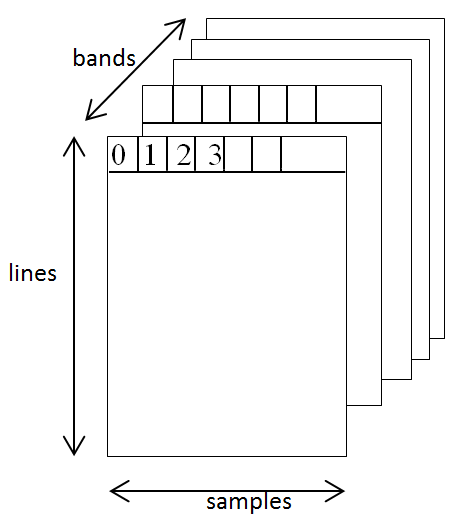
\includegraphics[width=\textwidth/5*2]{img/HI_bilFile}
		\caption[Hyperpsectral Cube]{This figure shows the order of the hyperspectral pixels saved into the the binary .bil file.}
		\label{fig:hyperspectralCube}
	\end{figure}
	
	The hyperspectral images also come with a number of drawbacks. A few are mentioned here but since hyperpsectral imagery is not the main focused of the thesis there are not addressed:
	\begin{itemize}
		\item System faults sometimes occurs and the affected areas are masked out. This results in blank areas. 
		\item As a passive sensor, it is dependent on the sun for illumination and thus vulnerable to poor weather conditions
		\item Due to the high refraction of light at some wavelengths, some bands are highly influenced by humidity (i.e. wavelength 1898.33nm).
	\end{itemize}
	
	To sum up, hyperpsectral images contain information beyond the visible and they are delivered in two files, one contains the hyperspectral cube and the other one the geo-locations of each pixel. In this project, they are used in Chapter \ref{Alignment}), where it is shown that the combination of Remote Sensing data confers better results for generating tree coverage maps. 
	
	
	
	
\end{document}
